\documentclass[tikz,convert={outfile=\jobname.svg}]{standalone}
\usepackage{pgf} 
\usepackage{amsmath}
\usepackage{ifthen}
\usetikzlibrary{positioning}

\begin{document}
\newcommand{\drawRCC}{
  
\begin{tikzpicture}
    \fill[black] (0,0) rectangle (3, 4);
    \clip (0,0) rectangle (3, 4); 
    \fill[gray] (0, 0.2) arc[start angle=-90, end angle=90, radius=1.8] -- cycle;
    \draw[white, ultra thick] (0, 0.2) arc[start angle=-90, end angle=90, radius=1.8];
    \node[white, anchor=north east, inner sep=2, outer sep=2] at (current bounding box.north east) {RCC};
    \draw[white, ultra thick] (0,0) rectangle (3, 4);
  \end{tikzpicture}
}

\newcommand{\drawMaskedRCC}[4]{
  \pgfmathsetseed{#1}
  \begin{tikzpicture}
    \fill[black] (0,0) rectangle (3, 4);
    \clip (0,0) rectangle (3, 4); 
    \fill[gray] (0, 0.2) arc[start angle=-90, end angle=90, radius=1.8] -- cycle;
    \draw[white, ultra thick] (0, 0.2) arc[start angle=-90, end angle=90, radius=1.8];
    \node[white, anchor=north east] at (3, 4) {RCC};
    \draw[white, ultra thick] (0,0) rectangle (3, 4);
    \foreach \x in {0, 1, 2} {
      \foreach \y in {0, 1, 2, 3} {
        \draw[white, very thin] (\x, \y) rectangle (\x+1, \y+1);
        \pgfmathsetmacro{\rand}{random}
        \ifdim \rand pt < \dimexpr#2 pt\relax
          \fill[#3, opacity=#4] (\x, \y) rectangle (\x+1, \y+1);
        \else
          \fill[black] (\x, \y) rectangle (\x+1, \y+1);
        \fi
      }
    }
  \end{tikzpicture}
}

\newcommand{\drawMLP}{
  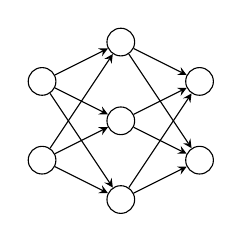
\begin{tikzpicture}
    % Input layer
    \foreach \i in {1, 2} {
      \node[circle, draw=black, fill=white, minimum size=10pt, inner sep=0pt] (input\i) at (0, -\i-0.5) {};
    }

    % Hidden layer
    \foreach \i in {1, 2, 3} {
      \node[circle, draw=black, fill=white, minimum size=10pt, inner sep=0pt] (hidden\i) at (1, -\i) {};
    }

    % Output layer
    \foreach \i in {1, 2} {
      \node[circle, draw=black, fill=white, minimum size=10pt, inner sep=0pt] (output\i) at (2, -\i-0.5) {};
    }

    % Connections from input to hidden layer
    \foreach \i in {1, 2} {
      \foreach \j in {1, 2, 3} {
        \draw[->, black, >=stealth] (input\i) -- (hidden\j);
      }
    }

    % Connections from hidden to output layer
    \foreach \i in {1, 2, 3} {
      \foreach \j in {1, 2} {
        \draw[->, black, >=stealth] (hidden\i) -- (output\j);
      }
    }
  \end{tikzpicture}
}

\newcommand{\drawFeatures}[3]{
  \begin{tikzpicture}
  \pgfmathsetseed{#1}
  \foreach \i in {0, ..., #2} {
    \node at (\i*0.8, 0) {
      $\color{#3}\scriptsize\begin{bmatrix}
        \pgfmathsetmacro{\rand}{rnd*9.9}
        \pgfmathprintnumber[fixed, precision=1]{\rand} \\
        \pgfmathsetmacro{\rand}{rnd*9.9}
        \pgfmathprintnumber[fixed, precision=1]{\rand} \\
        \vdots \\
        \pgfmathsetmacro{\rand}{rnd*9.9}
        \pgfmathprintnumber[fixed, precision=1]{\rand} \\
        \pgfmathsetmacro{\rand}{rnd*9.9}
        \pgfmathprintnumber[fixed, precision=1]{\rand}
      \end{bmatrix}$
    };
  }
  \end{tikzpicture}
}


\newcommand{\drawPosEnc}{
  \begin{tikzpicture}
  \node[circle, draw=black, minimum size=6cm] (circle) at (0, 0) {};
  \draw[black] (-3, 0) sin (-1.5, -1) cos (0, 0) sin (1.5, 1) cos (3, 0);
  \end{tikzpicture}
}
\tikzset{every picture/.style={/utils/exec={\sffamily}}}

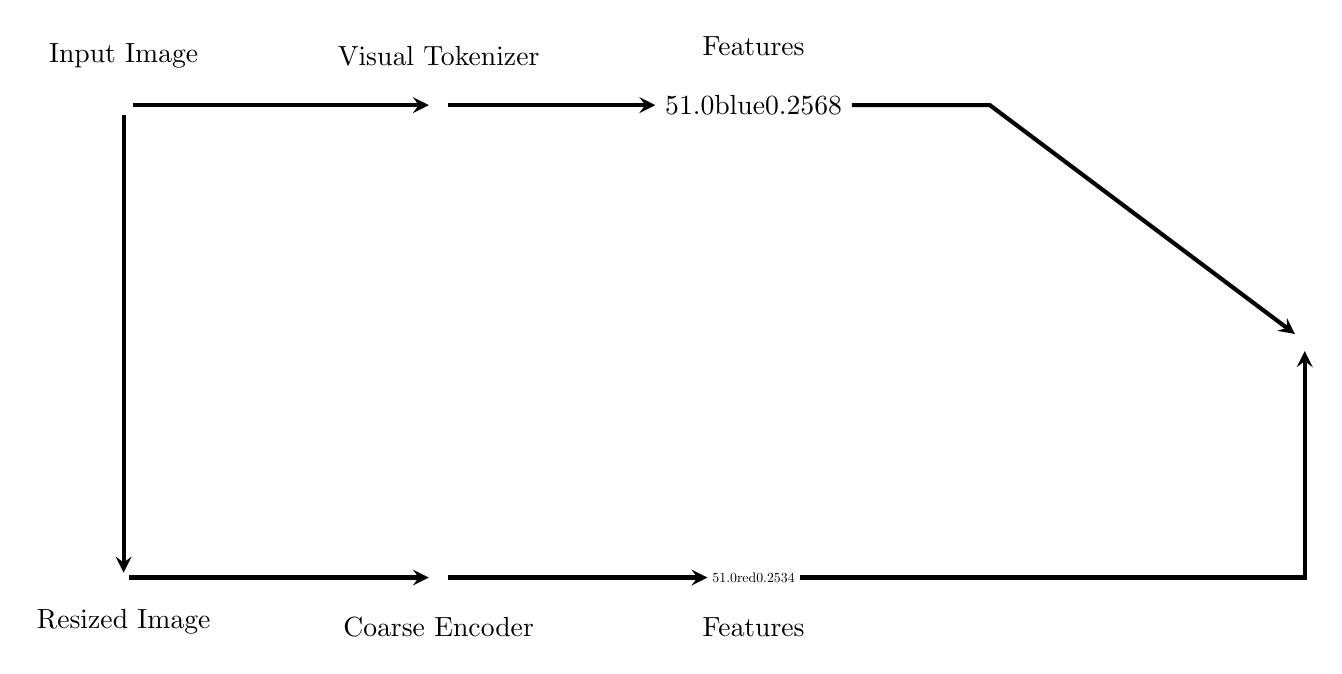
\begin{tikzpicture}
    % Input image with separate nodes for braces and arrows
    \node[name=rcc] at (0, 0){\drawRCC};
    \node[above=0.5cm of rcc.north, anchor=center] {Input Image};

    % Resized image (same approach)
    \node[name=resized, scale=0.5] at (0, -6){\drawRCC};
    \node[below=0.5cm of resized.south, anchor=center] {Resized Image};

    % Arrow with default spacing
    \draw[->, thick, black, >=stealth, line width=1.5pt] (rcc) -- (resized);

    % Coarse encoder
    \node[name=coarse_encoder] at (4, -6){\drawMLP};
    \node[below=0.5cm of coarse_encoder.south, anchor=center] {Coarse Encoder};
    \draw[->, thick, black, >=stealth, line width=1.5pt] (resized) -- (coarse_encoder);

    % Coarse features
    \node[name=coarse_features, scale=0.5] at (8, -6){\drawMaskedRCC{5}{1.0}{red}{0.25}{3}{4}};
    \node[below=0.5cm of coarse_features.south, anchor=center] {Features};
    \draw[->, thick, black, >=stealth, line width=1.5pt] (coarse_encoder) -- (coarse_features);

    % Visual tokenizer
    \node[name=visual_tokenizer] at (4, 0){\drawMLP};
    \node[above=0.5cm of visual_tokenizer.north, anchor=center] {Visual Tokenizer};
    \draw[->, thick, black, >=stealth, line width=1.5pt] (rcc) -- (visual_tokenizer);

    % Fine features
    \node[name=fine_features] at (8, 0){\drawMaskedRCC{5}{1.0}{blue}{0.25}{6}{8}};
    \node[above=0.5cm of fine_features.north, anchor=center] {Features};
    \draw[->, thick, black, >=stealth, line width=1.5pt] (visual_tokenizer) -- (fine_features);

    % Cross attention
    \node[name=cross_attention] at (15, -3){\drawMLP};
    \draw[->, thick, black, >=stealth, line width=1.5pt] 
        (fine_features) -- ++(3, 0) -- (cross_attention);
    \draw[->, thick, black, >=stealth, line width=1.5pt] 
        (coarse_features) -- ++(7,0) -- (cross_attention);




\end{tikzpicture}
\end{document}